\documentclass[11pt,a4paper]{article}
\usepackage[utf8]{inputenc}
\usepackage[T1]{fontenc}
\usepackage[serbian]{babel}
\usepackage[table,xcdraw]{xcolor}
\usepackage{array}
\usepackage{graphicx}
\usepackage{hyperref}
\hypersetup{
	colorlinks,
	citecolor=black,
	filecolor=black,
	linkcolor=black,
	urlcolor=black
}

\renewcommand*\contentsname{Sadr�aj}

\begin{document}

\begin{titlepage}

\centering
\textnormal{\large Elektrotehnicki fakultet Univerziteta u Beogradu}\\[0.1cm]
\textnormal{\large Prinicipi softverskog in�enjerstva}\\[3cm]

\textnormal{\normalsize - TIM Untitled(1).team -}\\\vspace{-5mm}
\rule{\textwidth}{0.4pt}
{\huge \bfseries SPECIFIKACIJA BAZE PODATAKA\\ 
za projekat Platforma za organizovanje volonterskih akcija\par}\vspace{-1mm}
\rule{\textwidth}{0.4pt}\\\vspace{1mm}
\textnormal{\large Autor: Ana Pe�ko}\\[6cm]


\includegraphics[scale=0.5]{logo.jpg}\\
\vfill
\textnormal{\normalsize Verzija 1.0}\\

\end{titlepage}

\tableofcontents

\newpage

\section{Uvod}
\subsection{Namena}
Baza podataka za projekat iz predmeta SI3PSI predstavlja fleksibilan i pouzdan nacin cuvanja podataka i pristupa istim od strane web servera radi generisanja web stranica.\par
U dokumentu su dati ER i IE modeli podataka, �ema relacione baze podataka, kao i opis tabela u bazi podataka.\par
Ovaj dokument slu�i kao osnova za razvoj detaljne projektne specifikacije posmatranog podsistema, implementaciju i testiranje.
\subsection{Ciljne grupe}
Dokument je namenjen vodi projekta i clanovima razvojnog tima. Vodi projekta dokument slu�i za planiranje razvojnih aktivnosti i specifikaciju imena tabela i imena polja u bazi, kako bi nezavisne celine, implementirane od strane razlicitih delova razvojnog tima, na kraju rada bile uspe�no integrisane.\par
Razvojnom timu dokument slu�i kao osnova za dizajn i implementaciju.
\subsection{Organizacija dokumenta}
Ostatak dokumenta organizovan je u sledeca poglavlja:
\begin{enumerate}
    \item \textbf{Model podataka} � model podataka u bazi i �ema baze
    \item \textbf{Tabele} � spisak tabela
\end{enumerate}
\subsection{Recnik pojmova i skracenica}
\begin{enumerate}
    \item IE � Information Engineering, notacija za modelovanje podataka
    \item ER � Entity/Relationship, notacija za modelovanje podataka
\end{enumerate}
\subsection{Otvorena pitanja}
\begin{center}
\begin{tabular}{| >{\centering\arraybackslash}m{1.9cm} | >{\centering\arraybackslash}m{4.9cm} | >{\centering\arraybackslash}m{4.9cm} |}
\hline
\rowcolor[HTML]{000000} 
{\color[HTML]{FFFFFF} Redni broj } & {\color[HTML]{FFFFFF} Opis } & {\color[HTML]{FFFFFF} Re�enje } \\ \hline
 &  & \\ \hline
 &  &  \\ \hline
 &  &  \\ \hline
 &  &  \\ \hline
\end{tabular}
\end{center}

\newpage

\section{Model podataka}
\subsection{ER notacija}
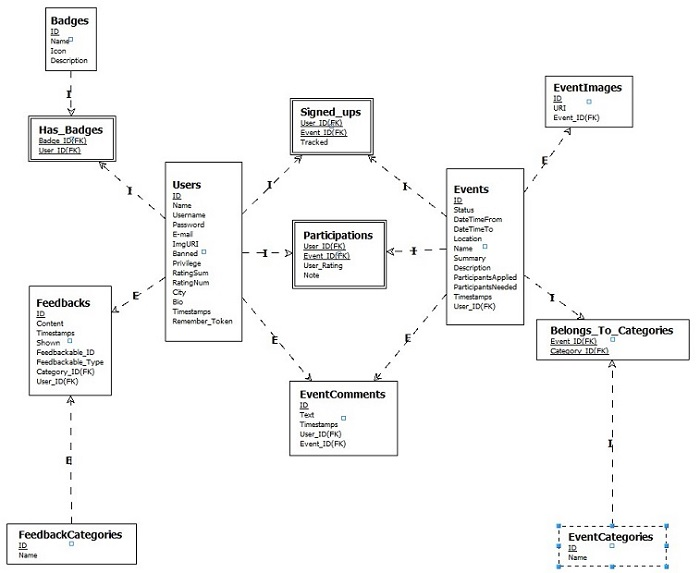
\includegraphics[scale=0.5]{ER-baza.jpg}\\

\subsection{IE notacija}
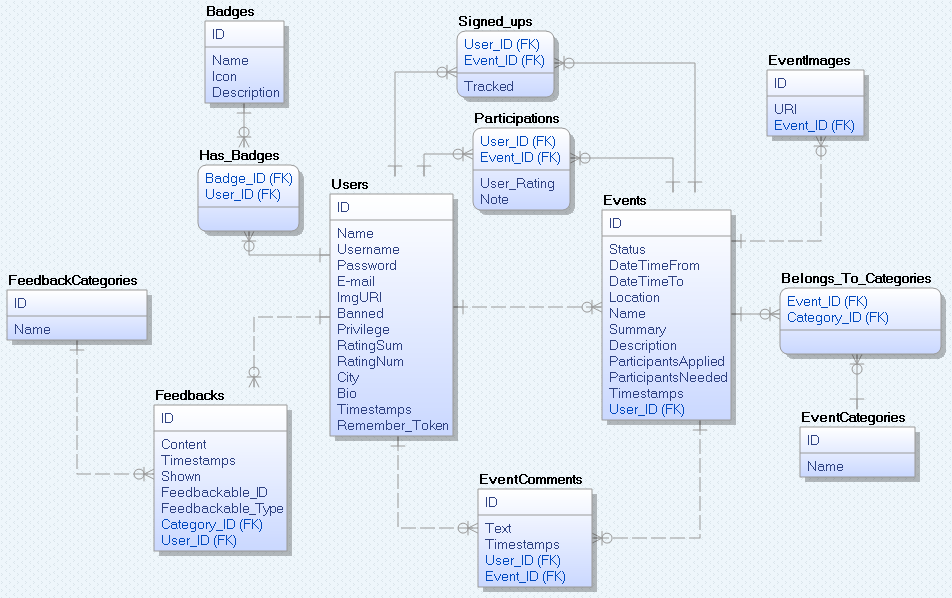
\includegraphics[scale=0.5]{evolDB_IEmodel.png}\\

\subsection{�ema relacione baze podataka}
\textbf{USERS}(ID, Name, Username, Password, Email, ImgURI, Banned,\\Privilege, RatingSum, RatingNum, City, Bio, Timestamps, Remember\_Token)\par
\textbf{BADGES}(ID, Name, Icon, Description)\par
\textbf{FEEDBACKCATEFORIES}(ID, Name)\par
\textbf{EVENTCATEGORIES}(ID, Name)\par
-----------------------------------------------------------------------------------------------\par
\textbf{EVENTS}(ID, User\_ID, DateTimeFrom, DateTimeTo, Location, Name, Summary, Description, ParticipantsApplied, ParticipantsNeeded, Status, \\Timestamps)\par
\textbf{EVENTIMAGES}(ID, URI, Event\_ID)\par
\textbf{EVENTCOMMENTS}(ID, Text, User\_ID, Event\_ID, Timestamps)\par
\textbf{FEEDBACKS}(ID, Content, User\_ID, Category\_ID, Shown,\\ Timestamps, Feedbackable\_ID, Feedbackable\_Type)\par
-----------------------------------------------------------------------------------------------\par
\textbf{BELONGS\_TO\_CATEGORIES}(Event\_ID, Category\_ID)\par
\textbf{HAS\_BADGES}(User\_ID, Badge\_ID)\par
\textbf{PARTICIPATIONS}(User\_ID, Event\_ID, User\_Rating, Note)\par
\textbf{SIGNED\_UPS}(User\_ID, Event\_ID, Tracked)

\newpage

\section{Tabele}
\subsection{USERS}
Sadr�i podatke o korisniku platforme.\par
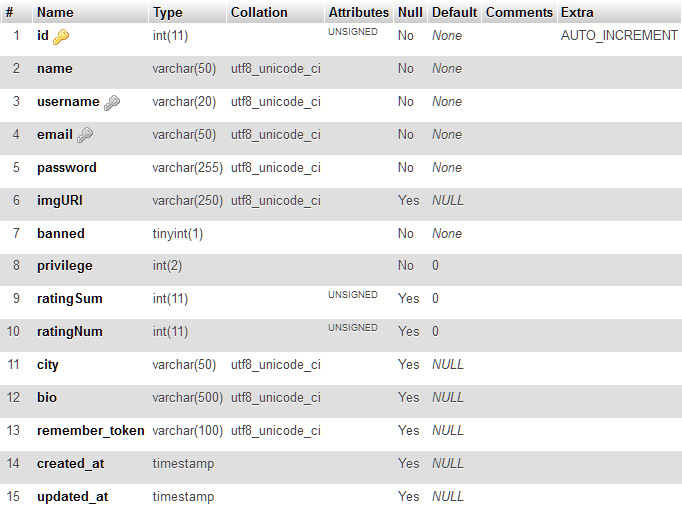
\includegraphics[scale=0.5]{USERS.png}\\

\subsection{BADGES}
Sadr�i podatke o svim bed�evima u sistemu.\par
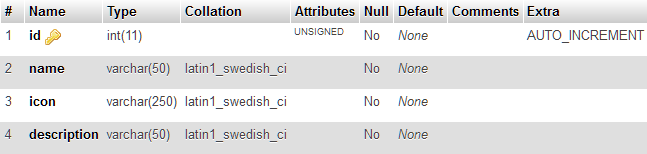
\includegraphics[scale=0.5]{BADGES.png}\\

\subsection{FEEDBACKCATEGORIES}
Sadr�i podatke o kategorijama povratnih informacija u sistemu.\par
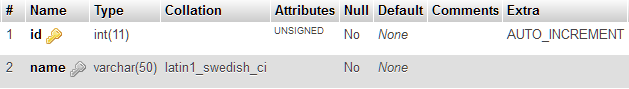
\includegraphics[scale=0.5]{FEEDBACKCATEGORIES.png}\\

\subsection{EVENTCATEGORIES}
Sadr�i podatke o kategorijama dogadaja u sistemu.\par
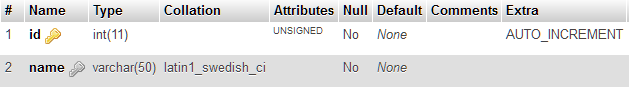
\includegraphics[scale=0.5]{EVENTCATEGORIES.png}\\

\subsection{EVENTS}
Sadr�i podatke o dogadajima u sistemu.\par
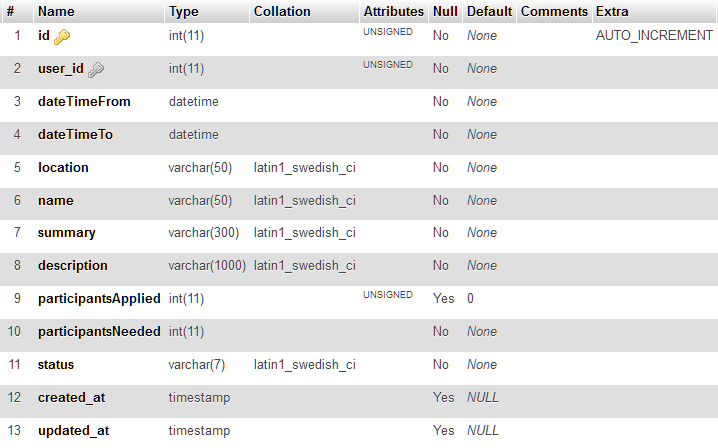
\includegraphics[scale=0.5]{EVENTS.png}\\

\subsection{EVENTIMAGES}
Sadr�i podatke o slikama vezanim za dogadaje u sistemu.\par
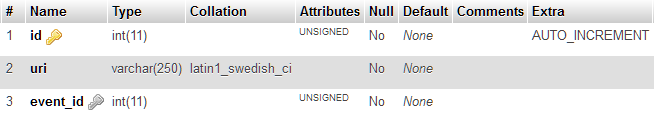
\includegraphics[scale=0.5]{EVENTIMAGES.png}\\

\subsection{EVENTCOMMENTS}
Sadr�i podatke o komentarima vezanim za dogadaje u sistemu.\par
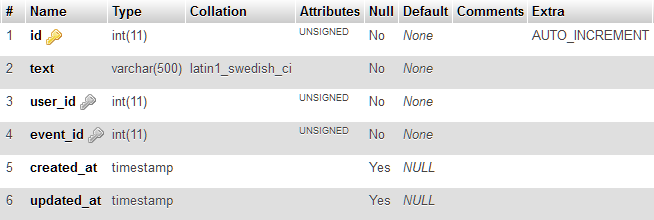
\includegraphics[scale=0.5]{EVENTCOMMENTS.png}\\

\subsection{BELONGS\_TO\_CATEGORIES}
Sadr�i podatke o tome kojim kategorijama pripadaju koji dogadaji.\par
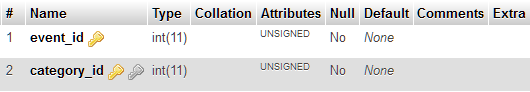
\includegraphics[scale=0.5]{BELONGS_TO_CATEGORIES.png}\\

\subsection{HAS\_BADGES}
Sadr�i podatke o tome koje bed�eve ima korisnik.\par
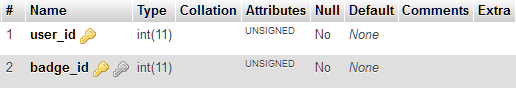
\includegraphics[scale=0.5]{HAS_BADGES.png}\\

\subsection{PARTICIPATIONS}
Sadr�i podatke koji su korisnici prisustvovali dogadaju.\par
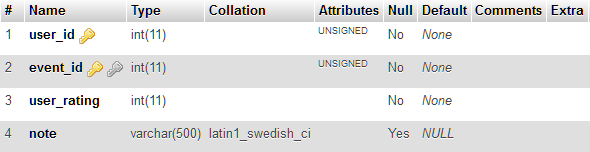
\includegraphics[scale=0.5]{PARTICIPATIONS.png}\\

\subsection{SIGNED\_UPS}
Sadr�i podatke koji su se korisnici prijavili za dogadaj.\par
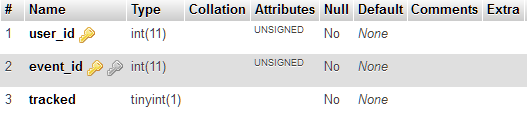
\includegraphics[scale=0.5]{SIGNED_UPS.png}\\

\newpage

\section{Spisak izmena}
\begin{center}
\begin{tabular}{| >{\centering\arraybackslash}m{2cm} | >{\centering\arraybackslash}m{1.3cm} | >{\centering\arraybackslash}m{4.2cm} | >{\centering\arraybackslash}m{4.2cm} |}
\hline
\rowcolor[HTML]{000000} 
{\color[HTML]{FFFFFF} Datum } & {\color[HTML]{FFFFFF} Verzija } & {\color[HTML]{FFFFFF} Opis } & {\color[HTML]{FFFFFF} Autor } \\ \hline
05.06.2016 & 1.0 & Osnovna verzija & Ana Pe�ko \\ \hline
 &  &  &  \\ \hline
 &  &  &  \\ \hline
 &  &  &  \\ \hline

\end{tabular}
\end{center}

\end{document}